
\section{Generatore di onda quadra}
	Per la realizzazione di un generatore di onda quadra si sono impiegati il multivibratore monostabile e astabile montati precedentemente, in modo da ottenere il circuito in \figurename{ \ref{f:qadra}}.

	\begin{figure}[H]
		\begin{minipage}{0.75\textwidth}
		\centering
		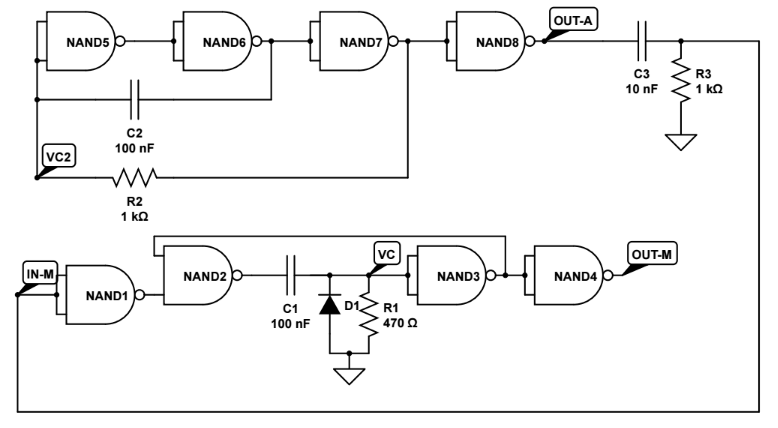
\includegraphics[scale=0.6]{../Figs-Tabs/qadra.png}
		\caption{schema del generatore di onde quadre}
		\label{f:qadra}
		\end{minipage}
		\begin{minipage}{0.14\textwidth}
			\begin{tabular}{l}
		$R_{3}=$\SI{988 \pm 8}{\ohm}\\
		$C_{3}=$\SI{10.8 \pm 0.4 }{\nano \farad}
			\end{tabular}
		\end{minipage}
	\end{figure}

	Si riporta in \figurename{ \ref{f:osci-qad}} l'acquisizione del segnale in
	ingresso nel multivibratore monostabile: il segnale in ingresso (ch1) e il segnale in uscita dal derivatore (ch2).

	\begin{figure}[H]
		\centering
		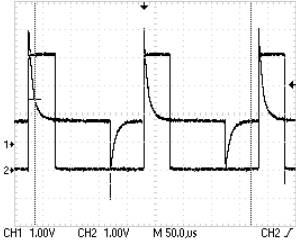
\includegraphics[scale=1.0]{../Figs-Tabs/deth_generator.png}
		\caption{input e output del multivibratore monostabile.}
		\label{f:osci-qad}
	\end{figure}

	Il circuito monostabile, come riscontrabile in \figurename{ \ref{f:osci-qad}},
	trasforma l'onda quadra generata dall'astabile in un impulso di breve durata temporale; sempre dalla figura in esame può essere osservato che il monostabile risulti sensibile al fronte di salita del segnale in ingresso.

	Come atteso, dall'andamento osservato in sezione 2, in uscita al circuito monostabile si ottiene un onda quadra [ch2 di \figurename{ \ref{f:osci-qad}}].
	Tale onda presenta un periodo
	$T=$\SI{205 \pm 1 }{\us}
	a fronte di un impulso di $\Delta T_{up} =$\SI{47.0 \pm 0.2 }{\us}. %\footnote[1]{} che è questo?
	Si ottiene pertanto un duty-cycle $\frac{\Delta T_{up}}{T}= 22.9 \pm 0.2$\textdiscount.

	Nella sezione 2 è stato osservato che l'impulso ,$\Delta T_{up}$,
	abbia una dipendenza lineare dal valore della resistenza $R_{2}$;
	la durata del periodo ne risulti indipendente; poiché non varia apprezzabilmente al variare di $R_{2}$.

	Mentre nella sezione  è stata osservata la dipendenza lineare
	del periodo $T$ dal valore della resistenza $R_{1}$;
	mentre la durata del impulso non vari significativamente.

	Si assume pertanto che $$ \Delta T_{up} \propto R_{2}$$
		$$T \propto R_{1} $$
	e non il viceversa.
	Per la verifica di tale assunzione si è proceduto a variare separatamente i valori di $R_{1}$ e $R_{2}$; si ottengono i dati in \tablename{ \ref{t:4}}.

	\begin{table}[htb]
		\centering
		\begin{tabular}{S[table-figures-decimal=0] S[table-figures-decimal=3] S[table-figures-decimal=0] S[table-figures-decimal=1] S}
			\toprule
			{$R_{1}$ [\si{\ohm}]} & {$R_{2}$ [\si{\kilo \ohm}]} & {$T$ [\si{\us}]} & {$\Delta T_{up}$ [\si{\us}]} & {$\frac{\Delta T_{up}}{T}$} \\
			\midrule
			470\pm 5	&	1.12 \pm 0.01	&	234 \pm 1	&	47.6\pm2	&	4.92 \pm3	\\
			567 \pm6	&	1.12 \pm 0.01	&	234\pm1	&	59.2 \pm4	&	3.95\pm 0.03	\\
			567 \pm6	&	0.988 \pm 0.009	&	205\pm1	&	59.2 \pm0.4	&	3.46\pm0.03	\\
			\bottomrule
		\end{tabular}
		\caption{
			Valori campionati per la verifica delle dipendenze di $\Delta T_{up}$ e $T$ dai valori di $R_{1}$ e  $R_{2}$.
		}
		\label{t:4}
	\end{table}
	Come possiamo osservare dai valori tabulati si ottiene un sostanziale accordo con la proporzionalità attesa.

	Si è adesso proceduto a realizzare un generatore di onde quadre di $T_{att}\sim 100$\si{\us} e $ \Delta {T_{up}}_{att}\sim 30$\si{\us}.

	Dai valori ottenuti nelle sezioni 2 e 3 e  dai rispettivi coefficienti stimati $a=$ e $b=$
		abbiamo stimato per i valori richiesti delle resistenze attese
	${R_{2}}_{att}=$\SI{470 \pm 30}{\ohm}%valore placeholder
	${R_{1}}_{att}=$\SI{260 \pm 40}{\ohm}%valore placeholder.
	Si è osservato tuttavia che impiegando tali resistori si ottiene un impulso sensibilmente diverso da quello atteso.
	Si è pertanto proceduto a variare i valori delle resistenze sino ad ottenere un accordo tra i valori misurati e quanto richiesto.
	Al termine di tale processo sono state impiegate delle resistenze
	$R_{1}=$\SI{331 \pm 3}{\ohm}
	$R_{2}=$\SI{464 \pm 4}{\ohm}
	ottenendo
	$T=$\SI{101 \pm 1}{\us} e $ \Delta {T_{up}}=$\SI{30.2 \pm 0.2}{\us}.

	Una posssibile causa della discrepanza tra i valori dei resistori, per cui si verifichi l'accordo con le richieste, ed  i valori di ${R_{2}}_{att}$ e 	${R_{1}}_{att}$ potrebbe essere imputabile ad un andamento non esattamente lineare nelle dipendenze di $ \Delta T_{up}$ da $ R_{2}$ e di
	$T $ da $ R_{1} $.
